\section{信号的描述和分类}

\subsection{信号的描述}

信号:信息的物理体现,随时间变化

分类:电信号/非电信号

基本形式:随时间变化的电压$v(t)$/电流$i(t)$\footnote{本课程内不区分电压信号和电流信号}

描述:时间的函数\footnote{本课程内信号和函数说法上等价},图形表示为波形

\subsection{信号的分类}

\begin{itemize}
    \item 用途:电视信号/雷达信号\dots
    \item 时间特性:确定/随机信号、连续\footnote{时间和幅值均连续}/离散\footnote{时间和幅值均离散,又称序列}信号、模拟/数字信号、周期/非周期信号、能量/功率信号\dots
\end{itemize}

\subsubsection{连续信号和离散信号}

\begin{Figure}[连续信号]
    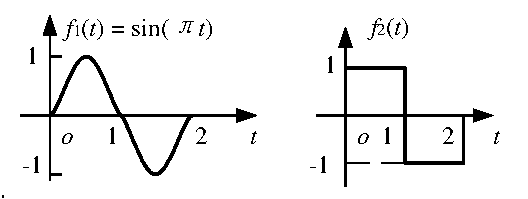
\includegraphics[width=80mm]{visio/1.2.pdf}
\end{Figure}

对于连续时间信号,其要求定义域连续,可包含间断点,值域可以不连续

\begin{Figure}[离散信号]
    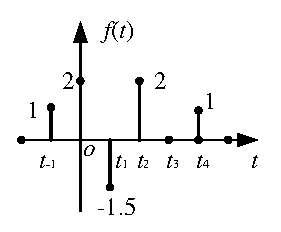
\includegraphics[width=40mm]{visio/1.3.pdf}
\end{Figure}

对于离散信号,其仅在离散时刻有定义,且离散点间隔可以不等,通常取间隔$T$,表示为$f(kT)$,简写为$f(k)$。

等间隔的离散信号称为序列,其中$k$为序号。

\xref{fig:离散信号}可以表示为以下形式:

\begin{equation}
    f(k)=\left\{
    \begin{aligned}
        1    & , & k=-1         \\
        2    & , & k=0          \\
        -1.5 & , & k=1          \\
        2    & , & k=2          \\
        0    & , & k=3          \\
        1    & , & k=4          \\
        0    & , & \text{其他}k
    \end{aligned}
    \right.
\end{equation}

\subsubsection{模拟信号、抽样信号和数字信号}

\begin{Figure}[模拟、抽样、数字信号]
    \begin{FigureSub}[模拟信号]
        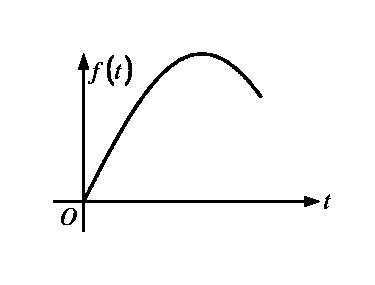
\includegraphics[width=40mm]{visio/1.4-a.pdf}
    \end{FigureSub}
    \begin{FigureSub}[抽样后信号]
        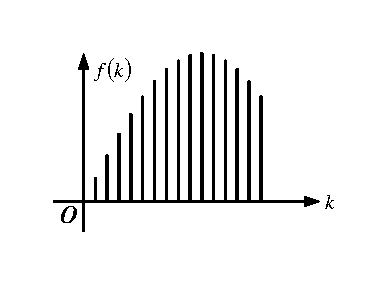
\includegraphics[width=40mm]{visio/1.4-b.pdf}
    \end{FigureSub}
    \begin{FigureSub}[数字信号]
        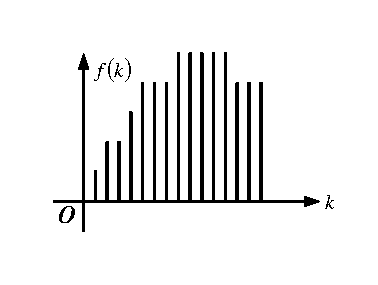
\includegraphics[width=40mm]{visio/1.4-c.pdf}
    \end{FigureSub}
\end{Figure}

对于模拟信号,其时间和幅值均连续,是连续时间信号,经过抽样后变换为抽样信号。

抽样信号时间离散但幅值连续,经过量化后变换为数字信号。

数字信号时间和幅值均离散,是离散时间信号。

\subsubsection{周期信号}

\begin{BoxDefinition}[周期信号]*
    定义在$(-\infty,\infty)$区间,每隔一定时间$T$(或整数$N$),按相同规律重复变化的信号。

    连续周期信号$f(t)$满足
    \begin{Equation}
        f(t) = f(t+mT), m=0,\pm 1,\pm 2,\dots
    \end{Equation}
    离散周期信号$f(t)$满足
    \begin{Equation}
        f(k) = f(k+mN), m=0,\pm 1,\pm 2,\dots
    \end{Equation}

    满足上述关系的最小$T$(或整数$N$)称为该信号的周期。
\end{BoxDefinition}

不具有周期性的信号称为非周期信号。

\begin{BoxProperty}[连续周期信号的周期]*
    两个周期信号$x(t),y(t)$的周期分别为$T_1$和$T_2$,若其周期之比$T_1/T_2$为有理数,则其和信号$x(t)+y(t)$仍然是周期信号,其周期为$T_1$和$T_2$的最小公倍数。
\end{BoxProperty}

\begin{BoxProperty}[正弦序列的周期]*
    对于离散周期信号$f(k) = \sin(\beta k)$。

    仅当$\frac{2\pi}{\beta}$为整数时,正弦序列才具有周期
    \begin{Equation}
        N=\frac{2\pi}{\beta}
    \end{Equation}
    当$\frac{2\pi}{\beta}$为有理数时,正弦序列仍具有周期性,其周期为
    \begin{Equation}
        N=M\cdot\frac{2\pi}{\beta}
    \end{Equation}
    其中$M$取使$N$为整数的最小整数。

    当$\frac{2\pi}{\beta}$为无理数时,为非周期序列。
\end{BoxProperty}

容易得知,两个周期信号的和不一定是周期信号,但两周期序列之和一定是周期序列。

\subsubsection{能量信号和功率信号}

\begin{BoxDefinition}[能量信号]*
    满足以下条件的连续信号称为能量信号
    \begin{Equation}
        E = \int_{-\infty}^{\infty}\left|f(t)\right|^2 dt < \infty
    \end{Equation}
    满足以下条件的离散信号称为能量信号
    \begin{Equation}
        E = \sum\limits_{k=-\infty}^{\infty}\left|f(k)\right|^2 < \infty
    \end{Equation}
    即能量有界,此时有$P = 0$
\end{BoxDefinition}

\begin{BoxDefinition}[功率信号]*
    满足以下条件的连续信号称为功率信号
    \begin{Equation}
        P = \lim_{T \rightarrow \infty} \frac{1}{T} \int_{-\frac{T}{2}}^{\frac{T}{2}}\left|f(t)\right|^2 dt < \infty
    \end{Equation}
    满足以下条件的离散信号称为功率信号
    \begin{Equation}
        P = \lim_{N \rightarrow \infty} \frac{1}{N} \sum\limits_{k=-\frac{N}{2}}^{\frac{N}{2}}\left|f(k)\right|^2 < \infty
    \end{Equation}
    即功率有界,此时有$E = \infty$
\end{BoxDefinition}

一般周期信号为功率信号,时限信号\footnote{有限时间区间不为零的非周期信号}为能量信号。

一些非周期信号也是非能量信号,例如:$\varepsilon (t)$ 是功率信号,$t\varepsilon (t)$、$e^t$是非功率非能量信号,$\delta (t)$是无定义的非功率非能量信号。

\subsubsection{一维信号和多维信号}

\begin{BoxDefinition}[一维信号]*
    只由一个自变量描述的信号,如语音信号。
\end{BoxDefinition}

\begin{BoxDefinition}[多维信号]*
    由多个自变量描述的信号,如图像信号。
\end{BoxDefinition}

\subsection{几种典型确定性信号}

\subsubsection{指数信号}

\begin{Figure}[指数信号]
    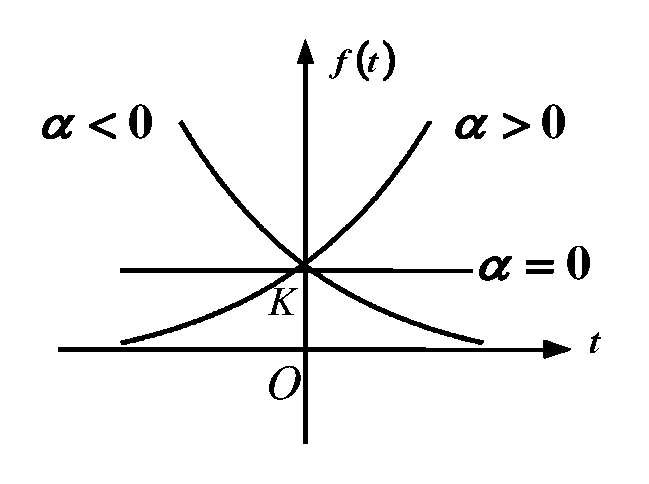
\includegraphics[width=40mm]{visio/1.5.pdf}
\end{Figure}

\begin{BoxDefinition}[指数信号]*
    形如以下形式的信号为指数信号
    \begin{Equation}
        f(t)=Ke^{\alpha t}
    \end{Equation}
    $\alpha = 0$时为直流(常数)

    $\alpha < 0$时指数衰减

    $\alpha > 0$时指数增长
\end{BoxDefinition}

\begin{BoxDefinition}[单边衰减指数信号]*
    \begin{Equation}
        f(t)=\left\{
        \begin{aligned}
            0    & , &t<0 \\
            e^{-\frac{t}{\tau}}    & , &t \geq 0
        \end{aligned}
        \right.
    \end{Equation}
    时间常数,代表信号的衰减速度
    \begin{Equation}
        \tau = \frac{1}{|\alpha|}
    \end{Equation}
\end{BoxDefinition}


\subsubsection{正弦信号}

\begin{BoxDefinition}[正弦信号]*
    形如以下形式的信号为正弦信号
    \begin{Equation}
        f(t)=K\sin(\omega t +\theta)
    \end{Equation}
    周期
    \begin{Equation}
        T = \frac{2\pi}{\omega}
    \end{Equation}
    角频率
    \begin{Equation}
        \omega = 2\pi f
    \end{Equation}
\end{BoxDefinition}

\begin{BoxDefinition}[衰减正弦信号]*
    \begin{Equation}
        f(t)=\left\{
        \begin{aligned}
            Ke^{-\alpha t}\sin(\omega t)    & , &t\geq 0 \\
            0    & , &t < 0
        \end{aligned}
        \right.
        \quad (\alpha > 0)
    \end{Equation}
\end{BoxDefinition}

\subsubsection{复指数信号}

\begin{BoxDefinition}[复指数信号]*
    复指数信号
    \begin{Equation}
        f(t)=Ke^{(\sigma + \mathrm{j} \omega)t}=Ke^{\sigma t}\cos(\omega t) + \mathrm{j}Ke^{\sigma t}\sin(\omega t)
    \end{Equation}
    复频率
    \begin{Equation}
        s=\sigma + \mathrm{j} \omega
    \end{Equation}
    其中$\sigma$的量纲为$1/s$,$\omega$的量纲为$rad/s$
\end{BoxDefinition}

特点:不能产生,用来描述各种信号,用于信号分析及运算简化。

当$\sigma = 0, \omega = 0$时,为直流信号

当$\sigma > 0, \omega = 0$时,为升指数信号

当$\sigma < 0, \omega = 0$时,为衰减指数信号

当$\sigma = 0, \omega \neq 0$时,为等幅振荡

当$\sigma > 0, \omega \neq 0$时,为增幅振荡

当$\sigma < 0, \omega \neq 0$时,为衰减振荡

\subsubsection{抽样信号}

\begin{Figure}[抽样信号]*
    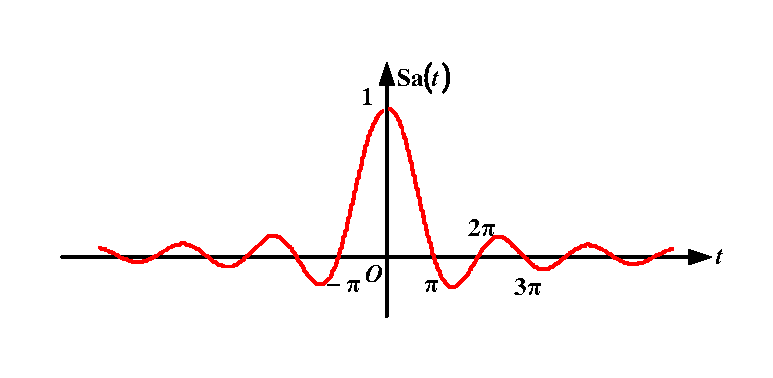
\includegraphics[width=100mm]{visio/1.6.pdf}
\end{Figure}

\begin{BoxDefinition}[抽样信号]
    抽样信号
    \begin{Equation}
        Sa(t)=\frac{\sin t }{t}
    \end{Equation}
\end{BoxDefinition}

\begin{BoxProperty}[抽样信号的性质]*
    抽样信号有如下性质
    \begin{Equation}
        \begin{array}{l}
            Sa(-t) = Sa(t) \\
            t=0,Sa(t)=1 \quad (\lim\limits_{t\rightarrow 0}Sa(t)=1)\\
            Sa(t)=0, t=\pm n\pi, n=1,2,3\cdots \\
            \int_0^{\infty}\frac{\sin t}{t}dt = \frac{\pi}{2}, \int_{-\infty}^{\infty}\frac{\sin t}{t}dt=\pi \\
            \lim\limits_{t\rightarrow\pm\infty}Sa(t)=0\\
            \mathrm{sinc}(t)=\frac{\sin(\pi t)}{\pi t}
        \end{array}
    \end{Equation}
    
\end{BoxProperty}

